\documentclass[]{style/ceurart}
\sloppy

% \documentclass{article}

\usepackage{booktabs}
\usepackage{multirow}
\usepackage{graphicx}
\usepackage{array}
\usepackage{caption}
\usepackage{listings}
\lstset{breaklines=true}

\begin{document}

\copyrightyear{2024}
\copyrightclause{Copyright for this paper by its authors.
  Use permitted under Creative Commons License Attribution 4.0
  International (CC BY 4.0).}

\conference{CLEF 2024: Conference and Labs of the Evaluation Forum, September 9-12, 2023, Grenoble, France}

\title{DS@GT eRisk 2024 Working Notes}

\author[1]{David Guecha}[
email=dahumada3@gatech.edu,
orcid=0009-0009-9855-5330
]
\author[1]{Aaryan Potdar}[
email=apotdar31@gatech.edu
]
\author[1]{Anthony Miyaguchi}[
orcid=0000-0002-9165-8718,
email=acmiyaguchi@gatech.edu,
]
\cormark[1]

\address[1]{Georgia Institute of Technology, North Ave NW, Atlanta, GA 30332}
\cortext[1]{Corresponding author.}


\begin{abstract}
In this document, we present our working notes for the eRisk lab of the CLEF 2024 competition, where we submitted entries for Task 1 and Task 3. For Task 1, we proposed two distinct pipelines for detecting signs of depression from millions of social media sentences, based on the 21 symptoms outlined in the BDI-II questionnaire. Our approach utilized both traditional NLP techniques, such as TF-IDF, and vector-based models. Specifically, we constructed a logistic regression classifier using the 21 symptoms as targets for a multiclass classification problem. Results on the hidden test set indicate that vector models and transformer-based models can achieve notable performance on information retrieval metrics, despite the absence of more complex sentence filtering and fine-tuning.

For Task 3, we employed simpler models, including XGBoost and Random Forests, which demonstrated better performance on smaller datasets.

\end{abstract}

\begin{keywords}
  Early Risk \sep
  Natural Language Processing \sep
  Machine Learning \sep
  Mental Health \sep
  Eating Disorders
\end{keywords}


\maketitle

\section{Introduction}

The eRisk Challenge 2024 comprises three distinct tasks aimed at developing early risk prediction systems that utilize social media documents to detect antisocial behaviors, signs of mental illnesses, and eating disorders. Predictions are made using state-of-the-art natural language processing techniques applied to user-generated content. Our team focused on two specific tasks: task 1, which involves identifying depression symptoms from a questionnaire, and task 3, which focuses on diagnosing eating disorders. For this challenge, we proposed a system that predicts symptoms of depression based on the Beck Depression Inventory (BDI-II) using various sentence processing architectures and a multi class classification approach. Additionally, we developed a system to predict symptoms of eating disorders by comparing vectors derived from sentence transformers to relevant symptoms and using simple models like XGBoost that work on smaller datasets as the one provided for task 3.



\section{Task 1: Search for symptoms of depression}

This task involves ranking documents relevant to symptoms of depression as identified in the BDI-II questionnaire. The objective is to submit runs containing the top thousand documents pertinent to a specific symptom. This is a standard information retrieval task commonly applied in search engines. The evaluation is conducted against a pool of human assessors who are experts in the field, categorizing sentences as either relevant or not relevant. There are two types of scoring: majority and unanimity (qrels).

For this year's task, qrels provided by human experts were made available, allowing these documents to be used as training data.


\subsection{Task 1: Related Work}

In previous iterations of this task, other teams have attempted to use vector representations of the sentences (formula ml 065)(uOttawa paper 069), and utilized either semantic search for transformer based models or cosine similarity to label the documents against the 21 symptoms of depression.


\subsection{Task 1 Methodology}

\subsubsection{Data management}
We collected the TREC formatted files and undertook extensive data cleansing, including the removal of special characters and the correction of formatting errors. Subsequently, we merged the cleaned files using a script that compressed the documents into the Parquet format, a binary format optimized for fast querying and favored over CSV and other formats for data engineering tasks.

To ensure both persistence and easy access during model development, we hosted the data in Google Cloud Buckets.

The dataset comprised both training and testing sets, with detailed statistics provided in Table 1. These posts were sourced from social media, and access to the data was facilitated through the Google Cloud API.


\begin{table}[]
\caption{Task 1 dataset statistics}
\begin{tabular}{llll}
             & Number of users & Number of sentences & Average number of words per sentence \\ \hline
Test set     & 551,311         & 15,542,200          & 17.98                                \\ \hline
Training set & 3,107           & 4,264,693           & 13.94                                \\ \hline
\end{tabular}
\end{table}



\subsubsection{Modeling}

Two distinct pipelines were employed for Task 1: a baseline pipeline and a sentence transformer-based solution. The system was hosted on Google Cloud Compute instances with the following specifications: Google Cloud Compute instance n1-standard-2. The code repository was maintained on GitHub.

The experiments were implemented in Python, utilizing the PySpark library for parallel processing and handling large data volumes. Luigi was used to define the data processing pipelines. 

For the models, we defined workflows using TF-IDF and Word2Vec, and employed Naive Bayes, logistic regression, and factorization machines for predictions. This allowed us to compare the performance of these traditional methods with the sentence transformer-based systems more details on table 2.

We ran three different models using traditional NLP techniques to generate sentence vectors from the documents: Word2Vec, TF-IDF, and Naive Bayes. Given the expected delays in retrieving embeddings with sentence transformers, we added a filtering step to the pipeline to reduce modeling time and computing costs. We used a count vectorizer to eliminate non-relevant posts, primarily spam or repeated strings.

To address this problem, we used relevancy labels (qrels) from previous competition years as binary inputs for a relevancy classification problem. We trained a classifier for each question to determine document relevancy to specific questions. Each document was evaluated against the classifier to obtain a relevancy probability, which was then used to rank the documents. The training data was vectorized using a count vectorizer, Word2Vec, and a text transformer. We hypothesized that framing the ranking task as a classification problem would yield satisfactory performance on the leaderboard. Additionally, we posited that unsupervised text representations with higher learning capacities would perform better in the relevancy classification task.

% \begin{table}
% \centering
% \begin{tabular}{llll}
% Model                                     & Description                                                                                                                                                                           &  &   \\
% Naive Bayes - Counting Vectorizer         & Discriminator based on feature-independence of words. Only usable with positive features.                                                                                             &  &   \\
% Logistic Regression - Counting Vectorizer & Classifier using vector of word counts, learns coefficients that determine how to weigh words to fit a decision boundary.                                                             &  &   \\
% Logistic Regression - Word2Vec            & Classifier using a word embedding that captures distributional semantics of the bag of words model. The unsupervised task should transfer knowledge to the simpler linear classifier. &  &   \\
% Logistic Regression - Text Transformer    & Classifier using the inductive properties of transformer layers to model a sequence of words in an auto-regressive manner.~                                                           &  &  
% \end{tabular}
% \end{table}

\begin{figure}[h]
\centering
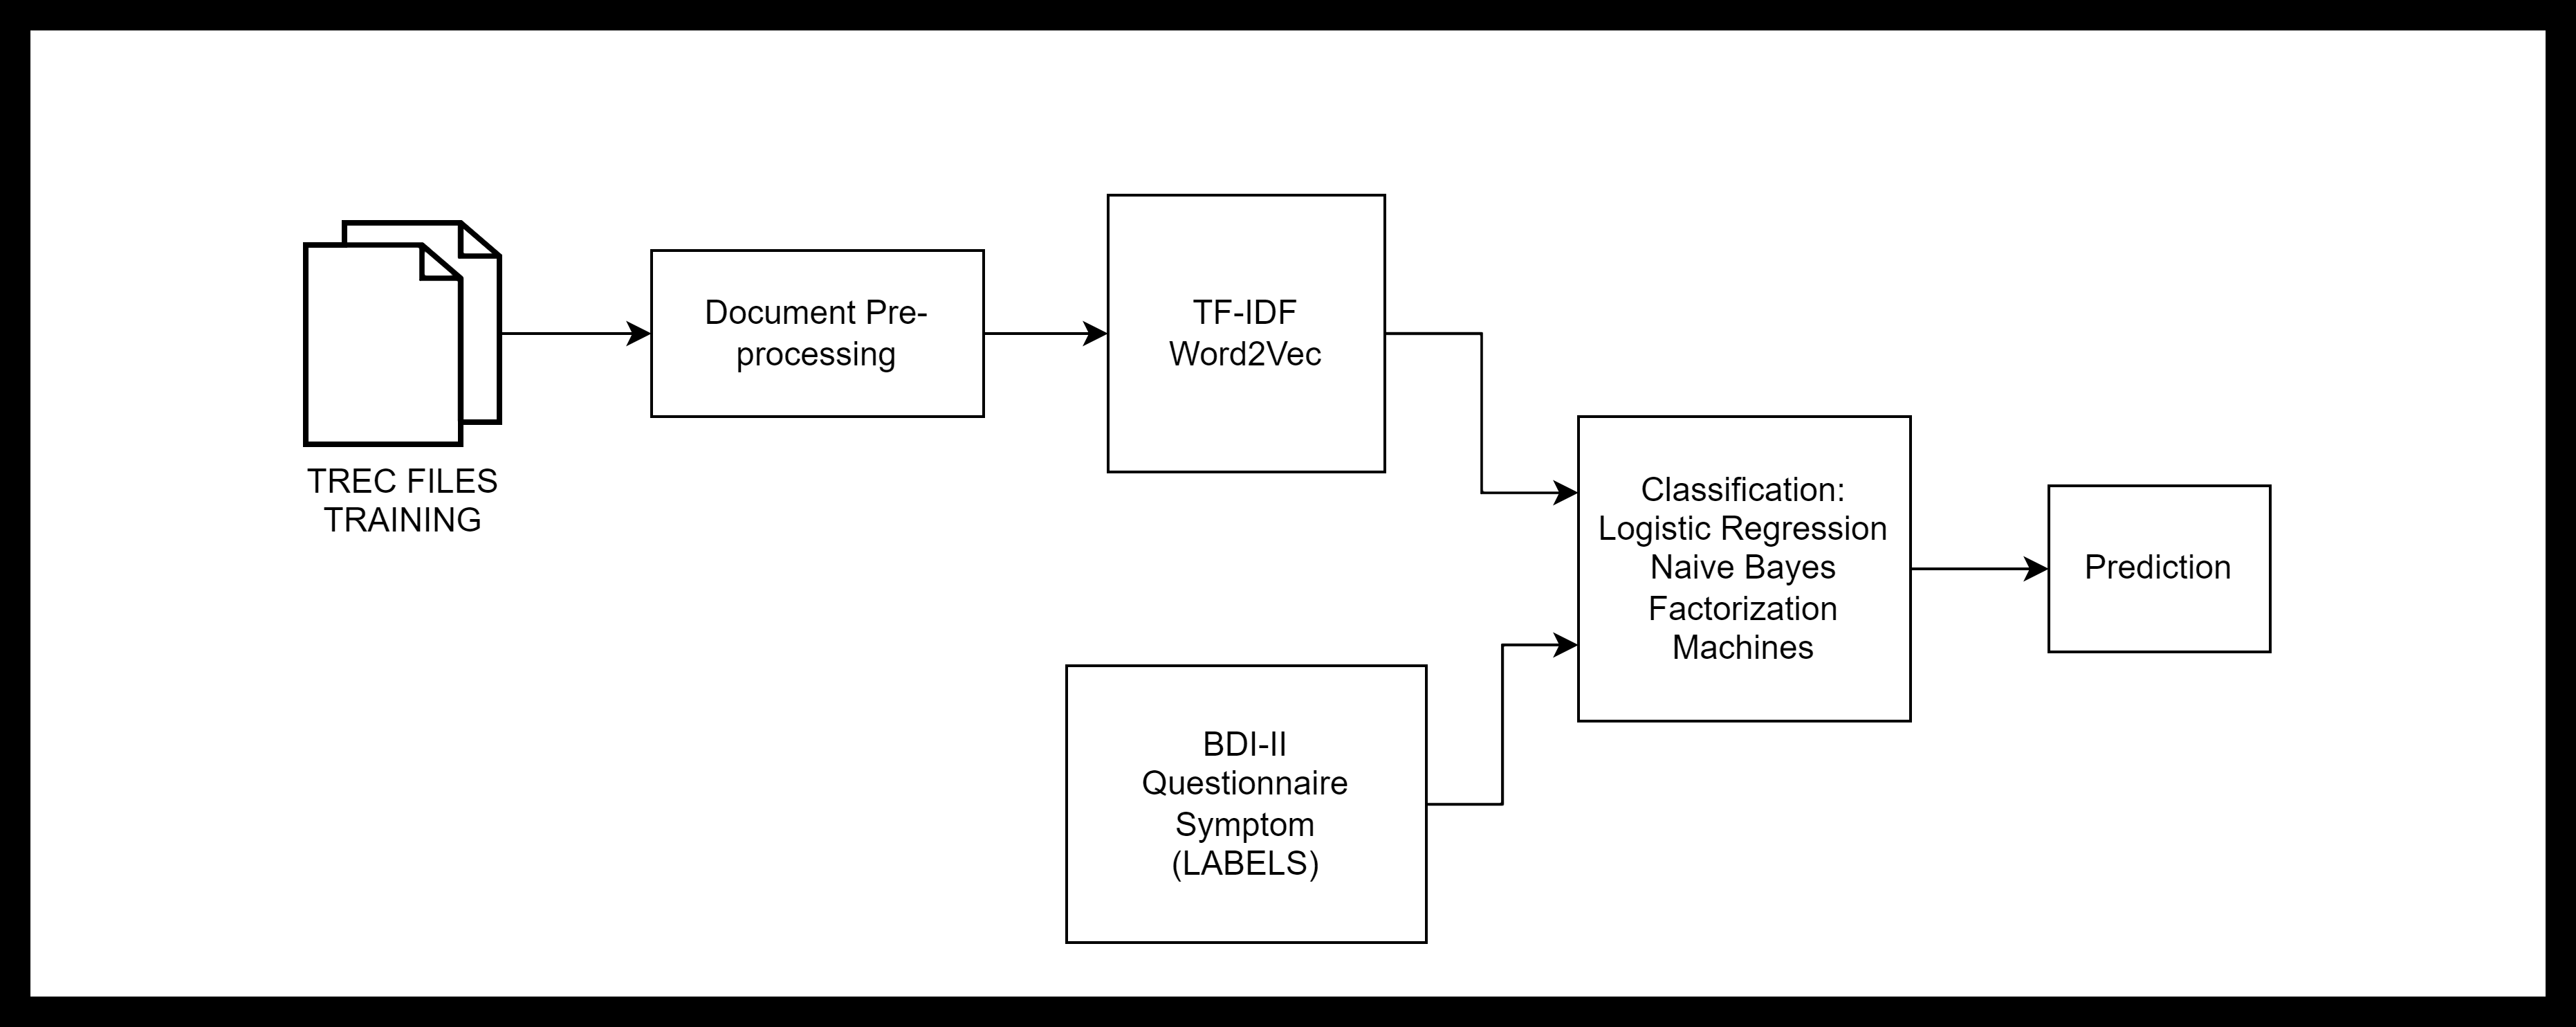
\includegraphics[width=\textwidth]{t1basepipeline.png}
\caption{Task 1 Base Pipeline}
\label{fig:example}
\end{figure}


\begin{figure}[h]
\centering
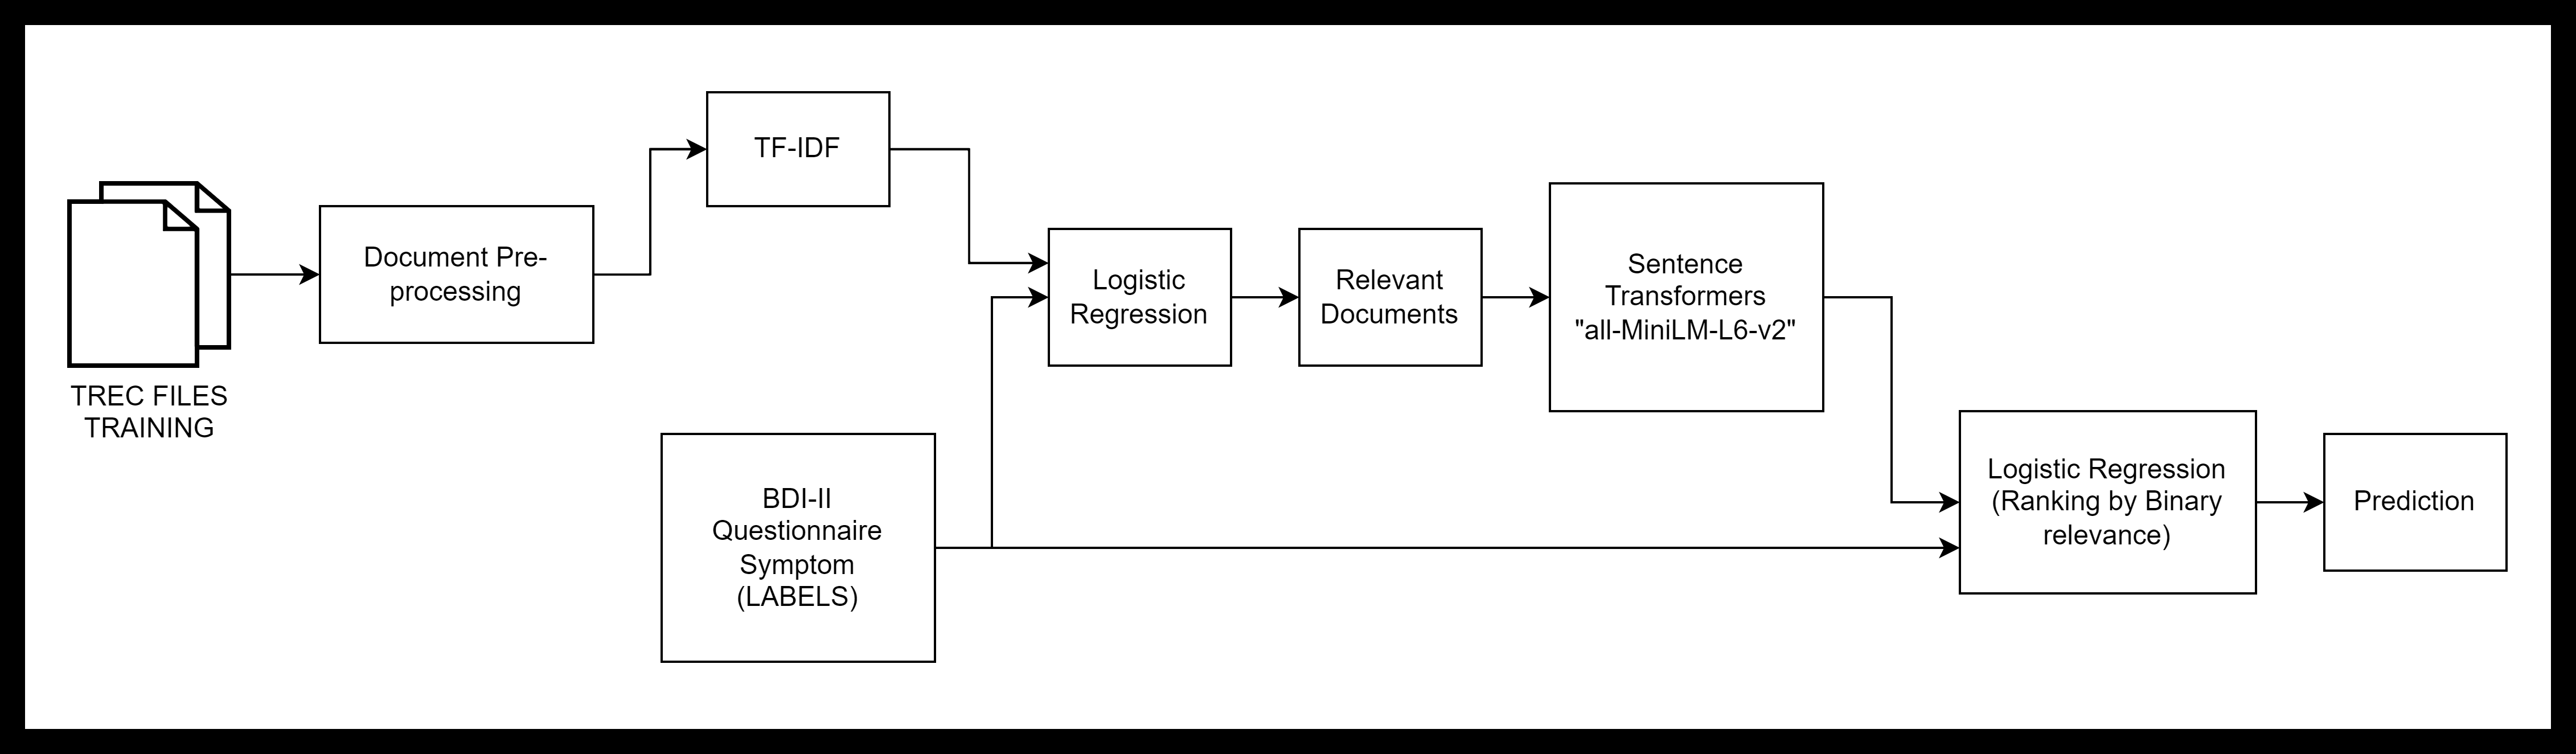
\includegraphics[width=\textwidth]{t1transformerspipeline.png}
\caption{Task 1 Transformers Pipeline}
\label{fig:example}
\end{figure}


\begin{table}
\centering
\caption{Modeling approaches}
\renewcommand{\arraystretch}{1.2}
\begin{tabular}{p{3in}p{3in}}
\toprule
\textbf{Model} & \textbf{Description} \\ \midrule
Naive Bayes - Counting Vectorizer & Discriminator based on feature-independence of words. Only usable with positive features. \\ \midrule
Logistic Regression - Counting Vectorizer & Classifier using vector of word counts, learns coefficients that determine how to weigh words to fit a decision boundary. \\ \midrule
Logistic Regression - Word2Vec  & Classifier using a word embedding that captures distributional semantics of the bag of words model. The unsupervised task should transfer knowledge to the simpler linear classifier. \\ \midrule
Logistic Regression - Text Transformer & Classifier using the inductive properties of transformer layers to model a sequence of words in an auto-regressive manner. \\ \bottomrule
\end{tabular}
\end{table}



\subsection{Task 1 Results}

% Please add the following required packages to your document preamble:
% \usepackage[table,xcdraw]{xcolor}
% Beamer presentation requires \usepackage{colortbl} instead of \usepackage[table,xcdraw]{xcolor}
% \usepackage[normalem]{ulem}
% \useunder{\uline}{\ul}{}
\begin{table}[]
\caption{Ranking-based evaluation for Task 1 (unanimity)}
\begin{tabular}{llllll}
Team & Run                       & MAP   & R-PREC & P@10 & NDCG  \\
\toprule
DSGT & logistic\_transformer\_v5 & 0.000 & 0.006  & 0.000                             & 0.010 \\
DSGT & logistic\_word2vec\_v5    & 0.000 & 0.001  & 0.000                             & 0.003 \\
DSGT & count\_logistic           & 0.000 & 0.000  & 0.000                             & 0.001 \\
DSGT & count\_nb                 & 0.000 & 0.000  & 0.000                             & 0.000 \\
DSGT & word2vec\_logistic        & 0.000 & 0.000  & 0.000                             & 0.000
\end{tabular}
\end{table}

\begin{table}[]
\caption{Ranking-based evaluation for Task 1 (majority voting)}
\begin{tabular}{llllll}
Team & Run                       & MAP   & R-PREC & P@10 & NDCG  \\
\toprule
DSGT & logistic\_transformer\_v5 & 0.000 & 0.009  & 0.000                             & 0.014 \\
DSGT & logistic\_word2vec\_v5    & 0.000 & 0.001  & 0.000                             & 0.003 \\
DSGT & count\_logistic           & 0.000 & 0.000  & 0.000                             & 0.001 \\
DSGT & count\_nb                 & 0.000 & 0.000  & 0.000                             & 0.000 \\
DSGT & word2vec\_logistic        & 0.000 & 0.000  & 0.000                             & 0.000
\end{tabular}
\end{table}



We find that after evaluation on the hidden test set, our models score near to zero nearly across the board. We find that the transformer-based model scores an order of magnitude more than the models without in the recall-precision and NDCG scores. 

\subsection{Task 1 Discussion}

We made a strong assumption in this project that a classifier could be repurposed into a functional ranker. 
Our results on the leaderboard show otherwise. 
One potential reason for the poor performance is the fact that learning a classifier that performs well on a specific metric (such as F1 or accuracy) does not mean that the model is well calibrated to the distribution of the actual data. 
If we had more time, we would have liked to explore proper ordinal regression through learning to rank.

We noted during the construction of the pipeline that there were a non-trivial number of training examples that had a high-degree of repetition. We would have liked to explore more options to reduce the number of relevant training examples. One potential solution to remove irrelevant documents would be to filter relevancy using a keyword-based information retrieval algorithm like BM25, before ranking the documents using a statistical model. These documents were a symptom of a poorly performing model, because they are ill-behaved degenerate examples that the model is not able to capture due to representation. For example, a word2vec model trained on a repeating fragment of “I AM SAD” will likely fall into the same semantic space as a single instance of the fragment, and would be difficult to differentiate from angle alone. This means that sentences with high compression ratios and low entropy should be filtered from the dataset. We found through qualitative evaluation during development that filtering out these specific sentences helped produce better retrievals.	


\subsection{Task 1 Future Work}

For future iterations of this task, we propose leveraging various language models to explore the capabilities of transformer-based systems. Additional strategies could include employing prompt engineering and using popular models to filter out sentences that are irrelevant to the symptoms. Given that large language models are regarded as the next evolution of search engines, this could prove to be a compelling area of exploration. Other potential avenues include fine-tuning language models and employing retrieval-augmented generation to enhance the accuracy of predictions.

\section{Task 3: Measuring the Severity of the Signs of Eating Disorders}

Eating disorders (ED) are serious mental health conditions characterized by abnormal eating habits. Early detection and severity assessment are crucial for timely intervention and treatment. The eRisk CLEF Task 3 aims to explore the feasibility of automatically estimating the severity of symptoms of ED using the Eating Disorder Examination Questionnaire (EDE-Q) based on the activity of social media users.

Users often view social media as an ideal platform for self-expression. They can share personal experiences and anecdotes while remaining anonymous to those on the platform. The openness of social media platforms allows users to easily seek support and advice from others without the fear of being judged. These factors make social media, such as Reddit, a valuable resource for mental health research. By analyzing the content shared by users, we can potentially identify early signs of eating disorders and assess their severity.


\subsection{Task 3 Overview}

For this task, participants were required to develop an automated system for predicting responses to an Eating Disorder Examination Questionnaire based on a history of their writings on Reddit. The EDE questionnaire is a 28-item self-reported questionnaire adapted from the Eating Disorder Examination (EDE). The questionnaire covers several domains such as dietary restraint, eating concerns, shape concerns, and weight concerns. Our goal was to predict the responses to 22 out of the 28 EDE-Q questions based on users' posting history. The responses range from 0 to 6, corresponding to the severity of symptoms.

The task is divided into two stages: training and test. Participants are provided with labeled training data to develop their models and unlabeled test data for evaluation. We aimed to leverage state-of-the-art NLP techniques and Machine Learning methods to design an automated pipeline for detecting the severity of the signs of EDs. We observed that our rather simple approach of BERT-based writing embeddings enabled us to achieve good performance with limited available information.


\subsection{Task 3 Dataset}

\begin{table}[h!]
\centering
\caption{Statistics for Task 3 dataset}
\begin{tabular}{|c|c|c|}
\hline
\multirow{4}{*}{2022} & No. of Subjects                 & 28     \\ \cline{2-3} 
                      & Min. no. of posts per Subject   & 12     \\ \cline{2-3} 
                      & Max. no. of posts per Subject   & 1143   \\ \cline{2-3} 
                      & Avg. no. of characters per Post & 184.33 \\ \hline
\multirow{4}{*}{2023} & No. of Subjects                 & 46     \\ \cline{2-3} 
                      & Min. no. of posts per Subject   & 5      \\ \cline{2-3} 
                      & Max. no. of posts per Subject   & 1161   \\ \cline{2-3} 
                      & Avg. no. of characters per Post & 223.25 \\ \hline
\end{tabular}
\end{table}

During the training phase of the challenge, the eRisk team released an entire history of user writings along with the corresponding answers to the EDE Questionnaire responses. The training data includes users from the 2022 and 2023 datasets, while the test data comprises new users from 2023. The combined training set consisted of 74 subjects. For each user or subject, we had access to a history of postings on Reddit and their responses to the EDE-Q questionnaire. We used the user responses as ground truth for training our machine learning models (discussed in the methodology section). The test set consisted of a history of postings for 18 users, structured similarly to the training set.



\subsection{Task 3 Methodology}

Our task is to predict the responses of the 2024 users to the EDE-Q questionnaire. To achieve this, we need to determine to what extent the characteristics associated with eating disorders are reflected in Reddit users' post and comment history. Note that the responses to the EDE-Q are integers ranging from 0 to 6. We approach this problem as a multi-class and multi-output classification task. The entire process is broken down into the following steps:

\subsubsection{Data Collection}

The datasets for the 2022 and 2023 users were provided by the eRisk team. This data was collected via web scrapers and outputted as XML files, with one JSON file corresponding to each user. We converted the acquired data to JSON format using BeautifulSoup and etree.XMLParser. The XML files contained appropriate tags, making the parsing process straightforward.

\subsubsection{Preprocessing}

Preprocessing involved converting the JSON files to readable DataFrames in Pandas and cleaning the text data to remove noise, such as URLs, hashtags, and special characters. We tokenized the text and applied NLP techniques such as lemmatization, stemming, and stopword removal to normalize the data.

Next, we leveraged the state-of-the-art BERT Large transformer model to generate writing embeddings. For this task, we used the `bert-base-uncased' pre-trained language model, which has been trained on 110 million parameters and works well with English texts. Writing embeddings were primarily generated in sentence chunks. For posts that were too long to feed into the transformer model (BERT has a maximum input sentence length of 512 tokens, including the [CLS] and [SEP] tokens), we concatenated all user posts together in chronological order and broke the resulting text into chunks of length \( n \), where \( n = 512 - 2 = 510 \). BERT produced embeddings with dimensions of 768.

\subsubsection{Feature Engineering}

Initially, we considered that the 768 dimensions of the sentence embeddings might be too large. Therefore, we standardized the features and conducted principal component analysis (PCA) for dimensionality reduction. The dimensions were reduced from 768 to 50. In the model training phase, we trained the machine learning models on both high-dimensional embeddings as well as embedding data obtained after dimensionality reduction.

\subsubsection{Modeling}

Since deep learning models require substantial amounts of data, we decided to use simpler machine learning models. We selected 5 models: Random Forest, Extra Trees, XGBoost, Ridge Regression, and Support Vector Machines (SVM). The models were trained using the generated embeddings.

\begin{table}[h]
\centering
\caption{Comparison of different classifiers}
\renewcommand{\arraystretch}{1.2}
\begin{tabular}{@{}lp{10cm}@{}}
\toprule
\textbf{Model} & \textbf{Description} \\ \midrule
Random Forest Classifier & Robust to Overfitting. Provides insights into feature importance. Versatile in handling categorical data. \\ \midrule
Extra Trees Classifier & Increased randomness for better generalization. Faster to train than Random Forests. \\ \midrule
XGBoost Classifier & Better performance on tabular data, due to gradient boosting framework. Built-in regularization to prevent overfitting. \\ \midrule
Ridge Classifier & Simple linear model. Incorporates L2 regularization to prevent overfitting. \\ \midrule
Support Vector Machine (SVM) & Effective for high-dimensional data. \\ \bottomrule
\end{tabular}
\end{table}

To evaluate the performance of the models, the eRisk team provided several evaluation metrics:
\begin{itemize}
    \item Mean Zero-One Error
    \item Mean Absolute Error
    \item Macro-averaged Mean Absolute Error
    \item Restraint Subscale
    \item Eating Concern Subscale
    \item Shape Concern Subscale
    \item Weight Concern Subscale
    \item Global ED (the global score)
\end{itemize}

For a model baseline, we used results from the runs for the 2023 challenge, which involved the same task.

\subsection{Task 3 Pipeline}

This pipeline outlines our approach to predicting EDE-Q responses based on users' social media activity, detailing the steps from data collection to model evaluation.

\begin{figure}[h]
\centering
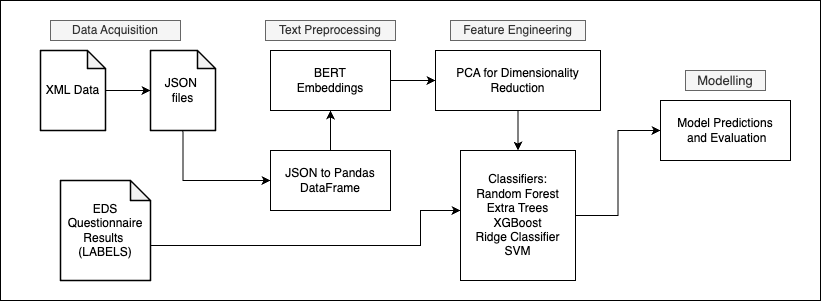
\includegraphics[width=\textwidth]{Task3Pipeline.png}
\caption{Task 3 Pipeline}
\label{fig:example}
\end{figure}

\subsection{Task 3 Results}

\begin{figure}[h]
\centering
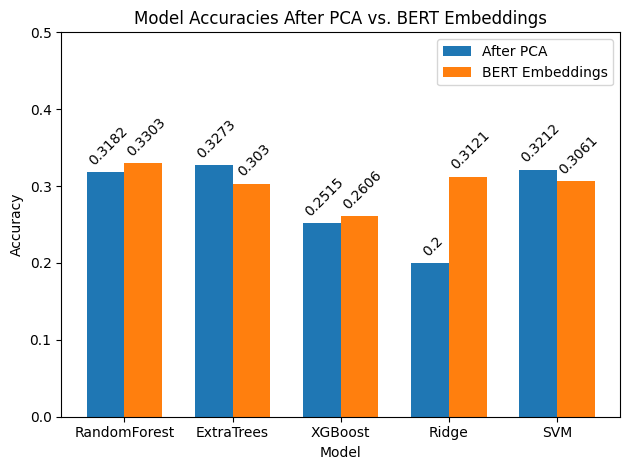
\includegraphics[width=0.8\textwidth]{task3ModelRes.png}
\caption{Task 3 Model performance on vector embedding with high dimensions and after dimensionality reduction.}
\label{fig:example}
\end{figure}

The results indicate that the Random Forest Classifier with high-dimensional embeddings performed the best overall, achieving an accuracy of 0.3303 and an MAE of 2.1091. This model benefited from the high-dimensional feature space, which likely captured the complex patterns in the data more effectively.

After applying dimensionality reduction, the Extra Trees Classifier emerged as the top performer with an accuracy of 0.3273. This suggests that reducing the feature dimensions helped in mitigating the curse of dimensionality and improving the model's generalizability.

Comparatively, the XGBoost Classifier showed lower performance across both feature sets, with an accuracy of 0.2606 and 0.2515 for high-dimensional and reduced-dimensional data, respectively. This may be due to the model's sensitivity to hyper-parameter tuning, which requires careful optimization.

The Ridge Classifier and SVM showed moderate performance. Notably, the Ridge Classifier's performance significantly dropped when trained on reduced dimensions data, with an accuracy of 0.2000, highlighting its limitation in handling reduced feature spaces effectively. The SVM performed consistently across both feature sets, but its overall accuracy remained lower compared to Random Forest and Extra Trees.

In summary, the Random Forest Classifier with high-dimensional data was the best overall model. However, after dimensionality reduction, the Extra Trees Classifier provided the best performance. Combining the results from both models through averaging indicated that the Random Forest model remained the best fit for this task.

\subsection{Task 3 Discussion}

\begin{table}[h]
\caption{Task 3 Results}
\begin{tabular}{llllllllll}
team     & run ID  & MAE   & MZOE  & MAEmacro & GED   & RS    & ECS   & SCS   & WCS   \\ \hline
baseline & all 0s  & 3.79  & 0.813 & 4.254    & 4.472 & 3.869 & 4.479 & 4.363 & 3.361 \\
baseline & all 6s  & 1.937 & 0.551 & 3.018    & 3.076 & 3.352 & 2.868 & 3.029 & 2.472 \\
baseline & average & 1.965 & 0.884 & 1.973    & 2.337 & 2.486 & 1.559 & 2.002 & 1.783 \\ \hline
DSGT     & 0       & 1.965 & 0.588 & 1.713    & 2.211 & 2.321 & 1.969 & 1.944 & 2.117
\end{tabular}
\end{table}

Our study achieved promising results in predicting the severity of eating disorder symptoms from social media content. While our models generally met baseline metrics, they significantly outperformed the baseline in Mean Zero-One Error (MZOE), Mean Absolute Error (MAE), and MAE macro metrics on the test data. However, our models fell short in meeting the baseline for the Eating Concern (ECS) and Weight Concern (WCS) subscales, suggesting a need for additional techniques like topic modeling or semantic analysis.

Despite these challenges, our team consistently ranked in the top 5 among five participating teams, with a total of 14 submissions. This highlights the robustness of our approach. Moving forward, further research should focus on refining our models and incorporating advanced techniques to enhance performance, ultimately contributing to improved interventions and support systems for individuals with eating disorders.

\subsection{Task 3 Future Work}

In the future, our research will focus on exploring the potential of deep learning models for predicting the severity of eating disorder symptoms from social media content. Deep learning architectures, such as recurrent neural networks (RNNs), offer the ability to capture complex patterns in text data more effectively, which could lead to improved performance.

Given that deep learning models often require large amounts of data, our next step will involve exploring data augmentation techniques. We plan to generate additional data using techniques such as Language Model Fine-Tuning (LMFT) or libraries like TextSynth, which can help increase the diversity and size of our dataset, thereby enhancing the robustness of our models.

Furthermore, to address the shortcomings in meeting the Eating Concern (ECS) and Weight Concern (WCS) subscales, we will incorporate semantic analysis techniques. By deepening our understanding of eating disorder sub-topics from textual data, we aim to refine our models and improve their ability to accurately assess the severity of specific symptoms. This approach will contribute to more comprehensive and precise predictions, ultimately enhancing the effectiveness of interventions and support systems for individuals with eating disorders.



Summary of the work and its contributions.

\section*{Acknowledgements}

Thank you to the DS@GT CLEF team for their support.

\bibliography{main}

% \appendix
% \section{Online Resources}

\end{document}